\documentclass[14pt]{extarticle}


%other%
\usepackage{graphicx}
\usepackage{float}
\usepackage[margin=0.5in]{geometry}
%other%


%math%
\usepackage{amsthm}
\usepackage{amsmath}
\usepackage{amssymb}
\usepackage{unicode-math}
\newtheorem*{lemma}{\textup{Лемма}}
\newtheorem*{corollary}{\textup{Следствие}}
\renewcommand\qedsymbol{$\blacksquare$}

\usepackage{parskip}

\usepackage{tikz}
   \usetikzlibrary{calc}

\newcommand{\arc}[0]{
   \tikz [baseline = (N.base), every node/.style={}] {
	  \node [inner sep = 0pt] (N){}; %{$#0$};
      \draw [line width = 0.8pt] plot [smooth, tension=1.3] coordinates {
         ($(N.north west) + (-1.5ex,0.6ex+0.4ex)$)
         ($(N.north)      + (-0.75ex,0+0.4ex)$)
         ($(N.north east) + (0ex,0.6ex+0.4ex)$)
      };
   }
}

\newenvironment{rcases}
  {\left.\begin{aligned}}
  {\end{aligned}\right\rbrace}



%math%

%fonts%
\usepackage[russian]{babel}
\usepackage{polyglossia}
\setdefaultlanguage[spelling=modern]{russian}
%\setotherlanguage{english}
\setmainfont{CMU Serif}
\setsansfont{CMU Sans Serif}
\setmonofont{CMU Typewriter Text}  
\setmathfont{Latin Modern Math}
%fonts%

\begin{document}


\begin{lemma}
	\textup{ 
	Окружности $\omega$ и $\Omega$ с радиусами 
	$R_1$ и $R_2$ вписаны в угол с вершиной $P$. %Известно, что $\omega \cap \Omega = \{M, N\}$. 
	Через $P$ внутри угла проведена произвольная прямая $k$.
	Пусть $k$ пересекает окружности 
	$\omega$ и $\Omega$ соответственно в точках $A$ 
	и $A'$; $B'$ и $B$. К окружностям в точках 
	$A$ и $B$ построены соответственно касательные $a$ и $b$.
	Пусть $a \cap b = C$. Тогда $AC = BC$. 
	}
\end{lemma}

\begin{proof}[\bf{\textup{Доказательство.}}]
	\begin{figure}[H]
	\centering
		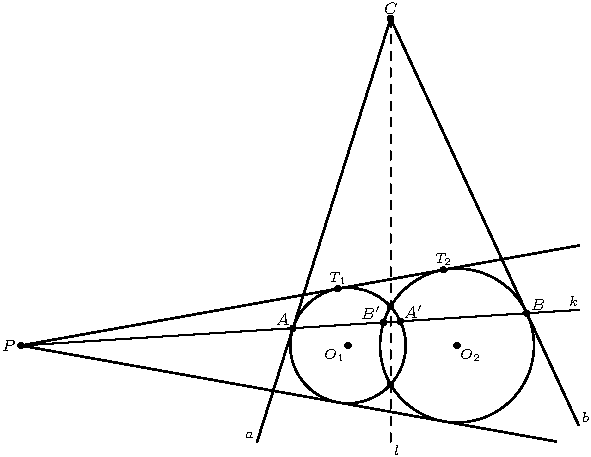
\includegraphics[height=12cm]{./img/img.pdf}
    \end{figure}
	Пусть $O_1$ и $O_2$ -- центры соответственно $\omega$ и $\Omega$.
    Заметим, что т.к. $\omega$ и $\Omega$ вписаны в один угол $\Rightarrow$ 
	$P$, $O_1$, $O_2$ лежат на одной прямой -- биссектрисе угла $P$.
	Зададим гомотетию $H_{P}^{\frac{R_2}{R_1}}$.
	Тогда $H_{P}(\omega) = \Omega$.\\
	Из свойств гомотетии имеем:
	\begin{equation*}
    \begin{rcases}
		H_{P}(A)      &= B'\\
		H_{P}(T_1)    &= T_2\\
		H_{P}(A')     &= B\\
	\end{rcases} 
    \text{$\Rightarrow \arc AT_1A' = \arc B'T_2B$}
    \end{equation*} 	

	Так как $\arc AT_1A' = \arc B'T_2B$, то по теореме об угле
	между касательной и хордой $\angle CBA = \frac{\arc B'T_2B}{2}
	= \frac{\arc AT_1A'}{2} = \angle CAB \Rightarrow \bigtriangleup
	ABC$ -- р/б $\Rightarrow AC = BC$.
	%Для начала заметим, что т.к. $\omega$ и $\Omega$ вписаны
	%в один и тот же угол, то $\bigtriangleup PO_1T_1 
	%\sim \bigtriangleup PO_2T_2$. Из подобия имеем:
	%$\frac{PT_1}{PT_2} = \frac{PO_1}{PO_2} = \frac{R_1}{R_2}$.
	%Рассмотрим $\bigtriangleup PO_1A$ и $\bigtriangleup PO_2A$.
	%Они подобны 
	
	%Пусть угол $\angle APT_1 = \alpha$, тогда $\angle \alpha = 
	%\frac{1}{2} ( \arc A'T_1 - \arc AT_1 )$
\end{proof}

\begin{corollary}
	\textup{
    Если $l$ -- радикальная ось окружностей $\omega$ и $\Omega$,
	то $C \in l$.
	}
\end{corollary}

\end{document}
